\documentclass[a4paper]{article}

%% Language and font encodings
\usepackage[english]{babel}
\usepackage[utf8x]{inputenc}
\usepackage[T1]{fontenc}
\usepackage[linesnumbered,lined,boxed,commentsnumbered]{algorithm2e}

%% Sets page size and margins
\usepackage[a4paper,top=3cm,bottom=2cm,left=3cm,right=3cm,marginparwidth=1.75cm]{geometry}

%% Useful packages
\usepackage{amsmath}
\usepackage{float}
\usepackage{graphicx}
\usepackage[colorinlistoftodos]{todonotes}
\usepackage[colorlinks=true, allcolors=blue]{hyperref}
\usepackage{subfig}
\usepackage{float}
\usepackage{amsmath}
\usepackage{caption}
\usepackage{adjustbox}
\usepackage{enumitem}

% Make lists more compact
\setitemize{noitemsep, topsep=0pt, parsep=0pt, partopsep=0pt}

\title{Computer Vision: Incisor Segmentation}
\author{Thierry Deruyttere (r0660485) \& Armin Halilovic (r0679689)}

\begin{document}
\maketitle



\section{Introduction}
This report describes our approach for automatic model based segmentation of incisor teeth in dental radiographs.
The approach mainly relies on ``Active Shape Modeling'', which is briefly explained in section~\ref{sect:asm}.
Then, in section~\ref{sect:preprocessing} we discuss how radiographs are preprocessed before model building and incisor detection is done.
Afterwards, we discuss two initialization and search methods we implemented and used in section~\ref{sect:init-estimate}.
Section~\ref{sect:evaluation} describes the formal performance evaluation procedure used for the results of the incisor segmentation process.
Experiments and results are be presented in~\ref{sect:experiments}.
We also did some experiments with neural networks, which are discussed in section~\ref{sect:nns}.
Finally, section~\ref{sect:conclusion} provides a conclusion of the work done.



\section{Active Shape Modeling (ASM)}
\label{sect:asm}
The idea behind ASM is to create a statistical model for a certain object which can be used to detect said object in unseen examples. 
The approach is explained in this section.
To create an active shape model, training data is needed. 
The training data should consist of images accompanied with landmark annotations.
These landmark annotations consist of $n$ points $({x_i, y_i})$ that indicate the object to be recognized.
The full landmark can be represented as a vector 
\begin{equation}
\textnormal{\textbf{l}} = (x_1, y_1, x_2, y_2, \ldots, x_n, y_n)^T
\end{equation}
A problem with landmark annotations across different images, is that they are not necessarily all at the same position nor do they have the same scale or rotation. This complicates the learning of the shape of the object we wish to detect. A solution for this is discussed below.

\subsection{Generalized Procrustes Analysis}
To train models using landmarks with different positions, scales, and rotations, the landmarks are first projected into the same normalized coordinate system. 
This is done by applying a ``Generalized Procrustes Analysis''.
The algorithm that does this can be seen in Algorithm \ref{algo:procr}.

\begin{algorithm}[!tbp]
\SetKwData{Left}{left}\SetKwData{This}{this}\SetKwData{Up}{up}
\SetKwFunction{Union}{Union}\SetKwFunction{FindCompress}{FindCompress}
\SetKwInOut{Input}{input}\SetKwInOut{Output}{output}
\Input{A list of landmarks}
\Output{A list of normalized landmarks}
\BlankLine

\For{$l$ in landmarks}{
	$l$ $\leftarrow$ translate $l$ such that its origin is (0,0) by subtracting the mean\;
    $l$ $\leftarrow$ rescale $l$ such that its scale is $1$\;
}
$ref$ $\leftarrow$ choose random reference landmark from landmarks\;
$converged \leftarrow false$\;
\While{not converged}{
	\For{$l$ in landmarks}{
    	$l$ $\leftarrow$ rotate $l$ towards $ref$\;
	}
$\bar{l}$ $\leftarrow$ calculate the mean landmark for all the landmarks\;
$d$ $\leftarrow$ distance between $\bar{l}$ and $ref$\;
$ref$ $\leftarrow$ $\bar{l}$\;
$converged \leftarrow d < threshold$\;
}
\Return{landmarks}
 \caption{Procrustes analysis}
 \label{algo:procr}
\end{algorithm}

\subsection{Principal Component Analysis (PCA)}
\label{subsect:pca}
Once all the landmarks have been projected into a normalized coordinate system, PCA is applied on them.
Applying PCA results in two matrices containing the eigenvectors and eigenvalues.
To create the statistical model, the top-$k$ eigenvectors are collected into a matrix $P$ and the mean landmark $\bar{l}$ is saved.
Using these eigenvectors and the mean landmark, a landmark $l$ can later be reconstructed with the following equations.
\begin{equation}
l \approx \bar{l} + Pb
\end{equation}
\begin{equation}
b = P^T (l - \bar{l})
\end{equation}
The vector $b$ in the equations above holds coefficients which are called the shape parameters.


\subsection{Matching the model on a new image}
When presented with a new image, we can apply the statistical model by first choosing an initial location where to put the model. 
How we derive this initial location is explained in section \ref{sect:init-estimate}.
Once this is done, the search procedure looks at a region around each landmark point in this initial estimate.
For each of these regions around a landmark points, a better points is chosen to replace the landmark point.
How these regions are viewed for each landmark point is described in the subsection below.
Once better landmark points have been chosen, the model can be matched to those points.
This is done by an iterative algorithm that updates the pose parameters scale, translation and rotation, and the shape parameters $b$~\cite{Cootes1992AnIT}.

\subsection{Grey Level Models}
\label{subsect:grey-level-models}
When we fit a model on a new image, we would like to detect the object we look for as well as possible.
To help this process, we use the training set to build a model that guides the search procedure.
For each of the landmarks in the training set, we build a grey level profile for each point $({x_i, y_i})$ of the landmark.
This is done is by sampling multiple points along the normal line for the point $({x_i, y_i})$ of the landmark.
For each of these sampled points, the grey level of the pixel they lie in is retrieved.
All of the grey values of these points are then stored in a vector \textbf{$g_i$}.
To reduce the effects of changes in global intensity, the derivative of each grey level profile is calculated~\cite{cootes1996statistical}.
The derivative of point $k$ in a grey level profile $j$ is calculated as
\begin{equation}
g'_{jk} = g_{jk+1} - g_{jk-1} 
\end{equation}
The derived profile will be denoted as $g'_j$. 
The derived profile is then normalized using the formula
\begin{equation}
g_j =\frac{g'_j}{\sum_k |g'_jk|}
\end{equation}

After the calculation of normalized grey level profiles for all the landmark points in all of the the different landmarks, the mean profile $\bar{g}_j$ is calculated for each landmark point $j$ of the landmarks, along with the covariance matrix $S_j$.
This is done under the assumption that the distribution of the grey level profiles follow a multivariate Gaussian distribution~\cite{Cootes1992AnIT}.
By calculating this covariance matrix and mean profile, we create a statistical model for each point.

The fit of a new profile is calculated by the ``Mahalanobis distance'' defined as
\begin{equation}
f(g) = (g-\bar{g_j})^TS_j(g-\bar{g_j})
\end{equation}
Finding the best new location for a point in the model is thus equivalent to minimizing the above distance metric.

To calculate a new profile $g$ for an unseen image, the model is first placed on an initialization position. Normal lines are then calculated for each point of the model, and grey level profiles are calculated at different points on each of these lines.



\section{Preprocessing}
\label{sect:preprocessing}
In order to improve the speed and efficiency of the segmentation process, images are preprocessed before they are used for model building and detection of teeth.

\subsection{Region of Interest Cropping}
First, to improve the speed of the whole process, images are cropped so that only the most relevant region remains.
This reduces the total preprocessing work that has to be done for a radiograph.
To determine to which region to crop, we looked at the radiographs that came with this project.
All of the radiographs looked very similar in a broad sense; the centers of the mouths always lied in a certain region of the image, and the scale was consistent across all images.
Because of this, we decided for the region of interest (ROI) to be a rectangle around the center of each image.
%Since all images were similar, we have determined the exact location of the ROI experimentally.
The values were chosen so that the ROI for each of the images would contain each of the eight incisor teeth along with a small buffer around the teeth.
The values we set for the ROI rectangle were 
\begin{align} 
(x_{start}, y_{start}) &= (x_{mid} - 375, y_{mid} - 450) \\ 
(x_{end}, y_{end})     &= (x_{mid} + 375, y_{mid} + 700)
\end{align}
This results in a region of 750 by 1150 pixels.
A drawback of this hardcoded approach is that a new radiograph which is shifted significantly will cause the segmentation process to not work correctly, since (a part of) the incisor teeth will then be cut off.

\subsection{Filters}
To preprocess images, we have tested many different filters.
The goal of using filters is to make teeth more visible in contrast to the rest of the image.
This should aid in the model building and tooth detection steps.
Making the teeth more visible than the mouth tissues also has a positive impact on the grey level models.
If the teeth are more visible than the rest, there will be a large difference in the grey levels at the edges of teeth.
The filters we eventually used are bilateral and contrast limited adaptive histogram equalization (CLAHE) filters.
These are applied on each image twice, each in alternating turns, starting with the CLAHE filter.
\bigskip 

The CLAHE filter is part of the family of adaptive histogram equalization (AHE) algorithms.
These algorithms are different than the normal histogram equalization algorithms as they compute histograms for different parts of an image instead of computing one histogram for the full image.
These histograms are then used to redistribute the lightness values over the whole image.
By doing this, we increase the local contrast and enhance edges in each region of the image.
However, these AHE algorithms tend to amplify noise in regions where the histogram is highly concentrated~\cite{AHE}. 
To avoid this we use the CLAHE filter which limits this amplification process.
CLAHE does this is by clipping the histogram at a predefined threshold.
The part of the histogram that is above this predefined threshold will then be evenly redistributed over the histogram.
The bilateral filter is then used to denoise the image by changing the intensity of each pixel by a weighted average of the intensity of the pixels around it.
The effect of applying these filters can be seen in Figure~\ref{fig:preprocessing} (a), (b) and (c).
% Ge kunt ni "we have tried many different filters" zeggen en dan maar praten over 2 he
We have also considered the use of adaptive threshold filters and Sobel filters to increase the contrast between the teeth and the rest of the images or to make their edges much clearer, but did not manage evaluate their effects in the time allocated to this project.

\subsection{Gaussian Pyramid}
\label{subsect:gaussian-pyramid}
For the implementation of a multi resolution search algorithm, a Gaussian pyramid of images is created.
This is a pyramid of a predetermined number of levels.
The pyramid starts at level 0, which contains the original image.
Each higher level then contains a downsampled image of the level before it using a Gaussian average.
Each pixel at a higher level contains a local average of a pixel neighborhood on the level below it in the pyramid.
Figure~\ref{fig:preprocessing} (d) shows a radiograph after the preprocessing step.
\begin{figure}[H]
    \centering
        \subfloat[The cropped image of radiograph ``01.tif''.]{{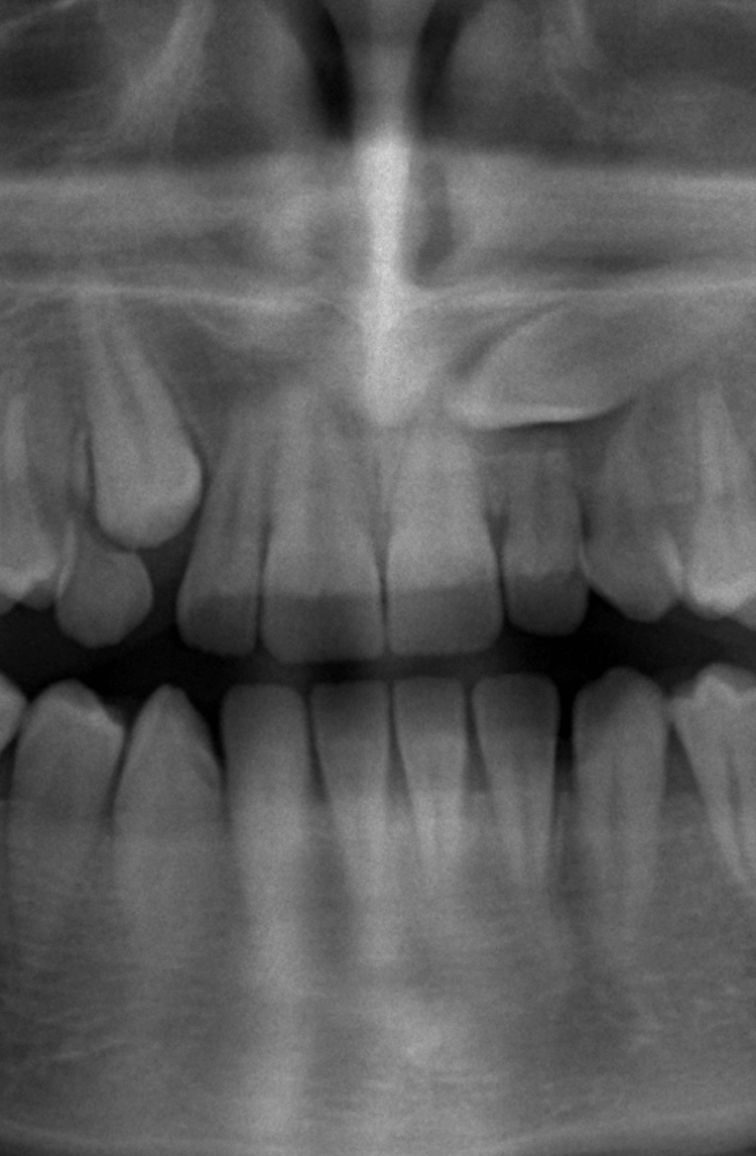
\includegraphics[width=5cm]{orig-1}}}
    \qquad
    \subfloat[The image after applying CLAHE and bilateral filter once.]{{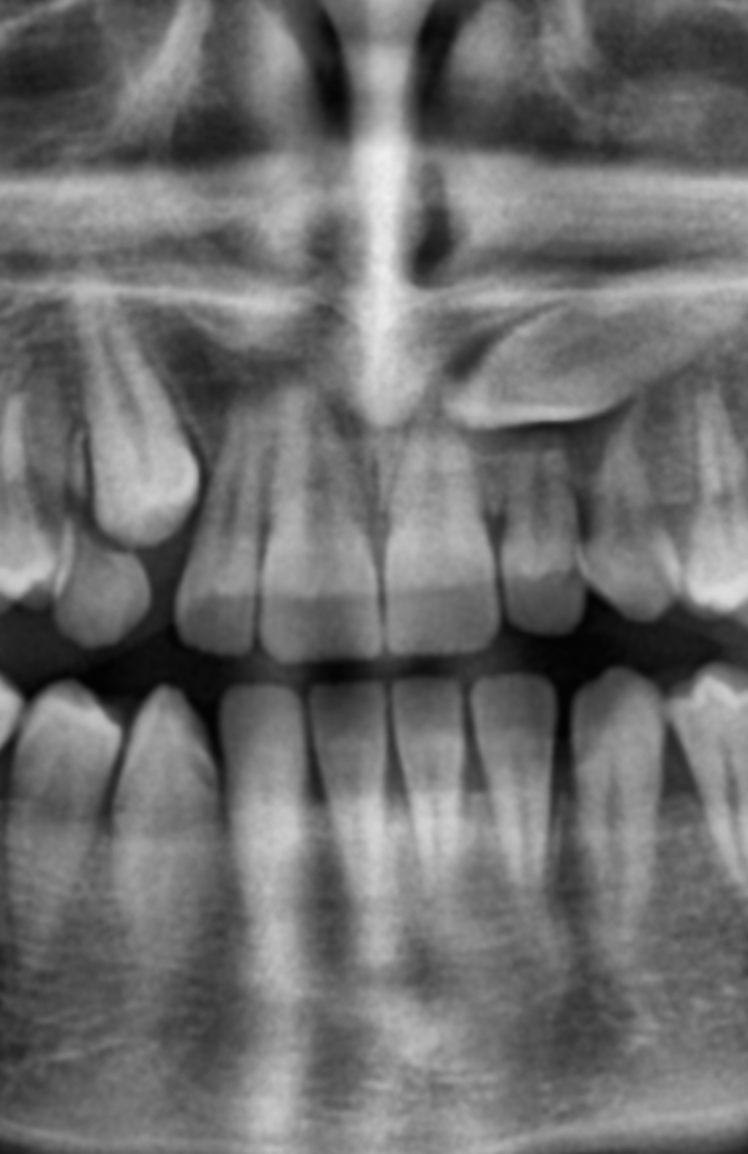
\includegraphics[width=5cm]{preprocessed-1}}}
    \qquad
    \subfloat[The image after applying CLAHE and bilateral filter twice.]{{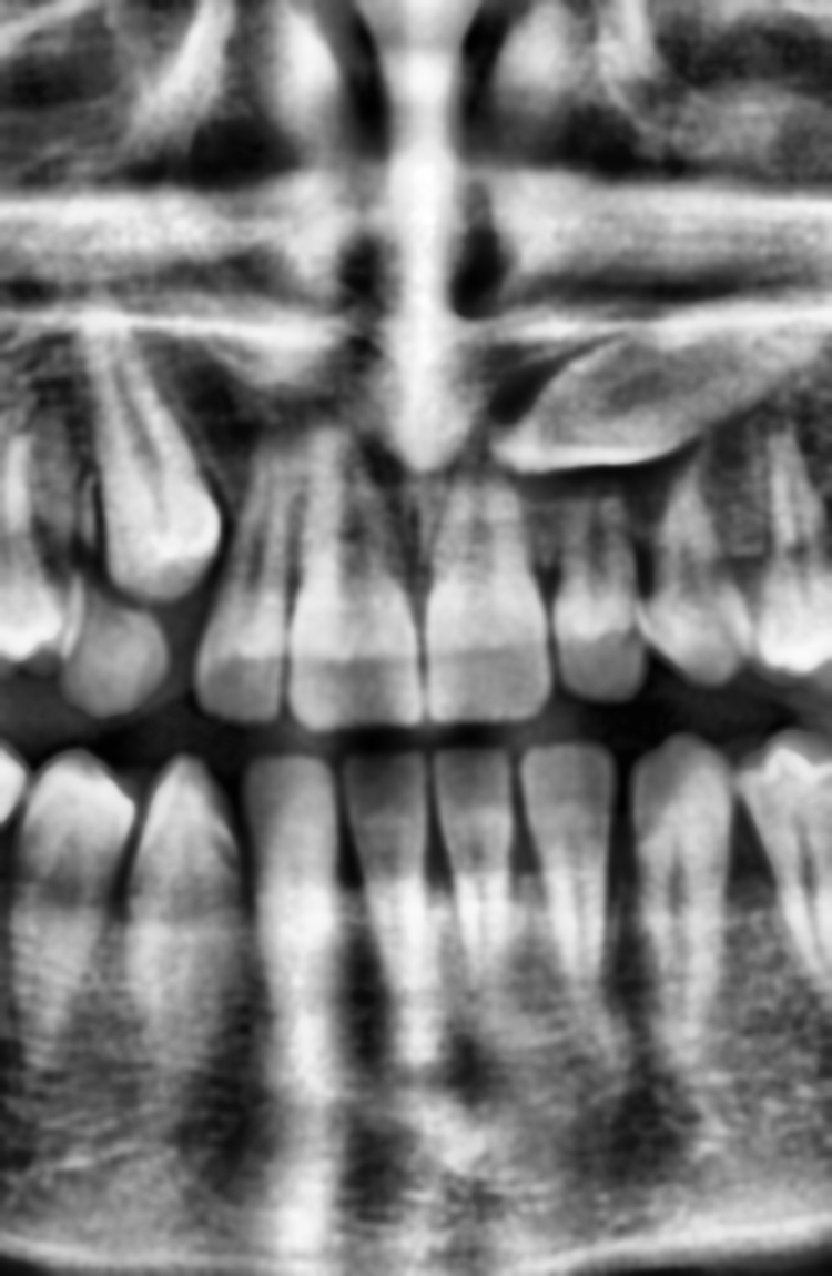
\includegraphics[width=5cm]{radiograph-01-preprocessed-level-0.png}}}
    \qquad
    \subfloat[The image after applying CLAHE and bilateral filter twice and moving three levels higher in the Gaussian pyramid.]{{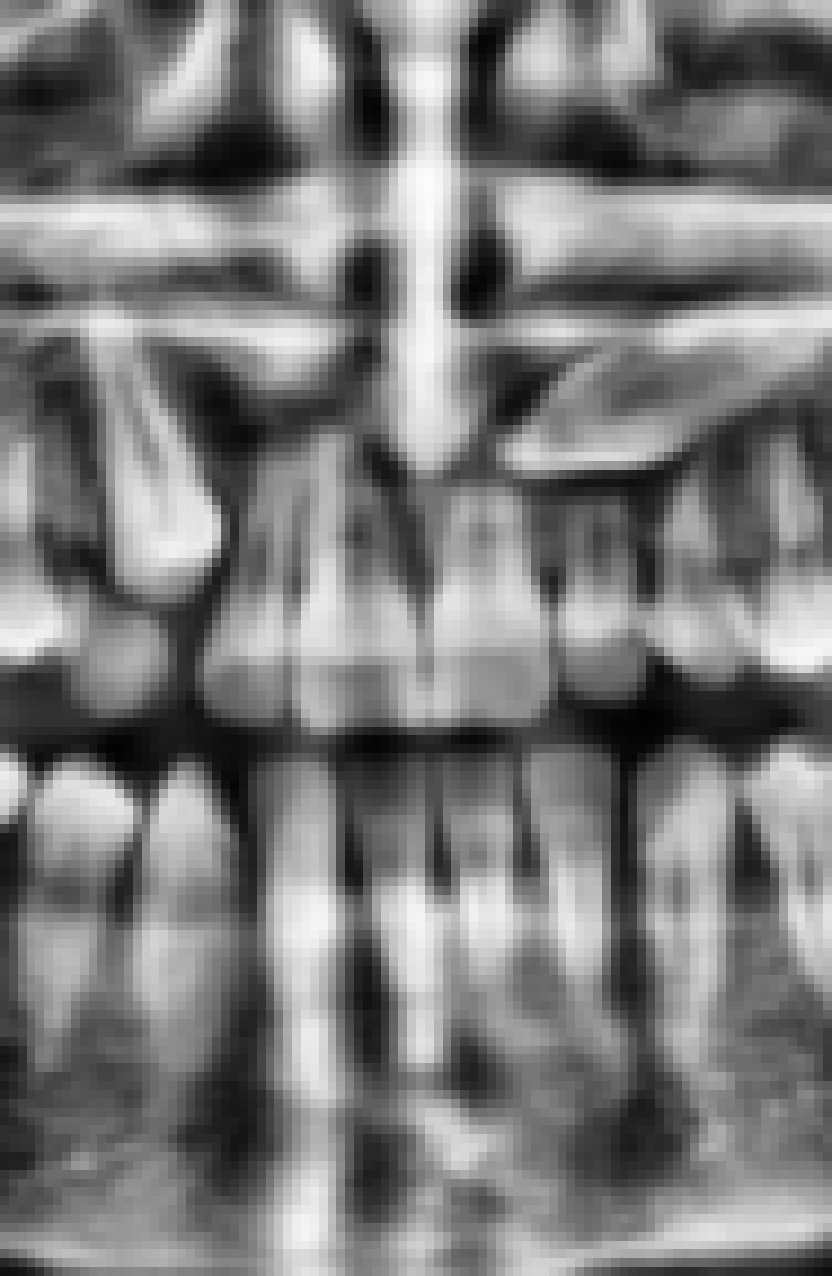
\includegraphics[width=5cm]{radiograph-01-preprocessed-level-3.png} }}
    \caption{The effects of applying the different filters.}
  \label{fig:preprocessing}
\end{figure}



\section{Fitting a model to an image}
\label{sect:init-estimate}
This section describes the two approaches that were used for the initial positioning of a tooth model and the following search procedure to fit the model to an image.
The first approach (subsection~\ref{subsect:upper-lower-incisors}) makes use of an ASM for the upper four incisor teeth and another one for the lower four incisor teeth.
When those models converge, individual teeth are detected using models for individual teeth.
The second method (subsection~\ref{subsect:multi-res}) uses a multi resolution ASM for both the initialization and complete incisor detection.
Both of these methods rely on finding the center of the mouth for the initialization step, which is explained first.

\subsection{Locating the center of a mouth}
\label{subsect:center of mouth}
In order to find the $y$ center of a mouth, a dynamic programming approach was implemented to find a line that can split the two jaws of the mouth.
Since the area between two jaws is one of the darkest regions on the preprocessed radiographs, we opted to find a line that travels through this dark area from left to right.
Such a line, which we named the ``jaw split line'', is discovered using the Viterbi algorithm. 
To speed up the search we decided to only search for this ``jaw split line'' in a region around the vertical center of each ROI.
The region is described by the following variables:
\begin{align} 
y_{search\_min} &= y_{roi\_max} / 2 - 300\\ 
y_{search\_max} &= y_{roi\_max} / 2 + 200
\end{align}
The Viterbi search starts on the leftmost $x$ position of each ROI with each of the $y$ values in the region initialized to the intensity of the pixels in the ROI.
The algorithm searches for the darkest path one $x$ position at a time.
For each next $x$ position, it loops over each $y$ position and looks at the best (i.e. lowest intensity) previous $y$ position that can reach the current $y$ position.
The algorithm has been set to move forward in the path by 10 pixels at each iteration, and to look in a window of 10 previous $y$ positions to find the next best $y$ position.
These settings are used to create a speed up for the algorithm.
Figure~\ref{fig:jawSplitLine} shows two jaw split lines.
The left one is the split line in a relatively simple case; the black area between the jaws follows a fairly straight path. 
However, in the right one the black area is not straight at all, but the Viterbi approach still manages to find a good jaw split line in this case.

\begin{figure}[!tbp]
    \centering
    \subfloat[]{{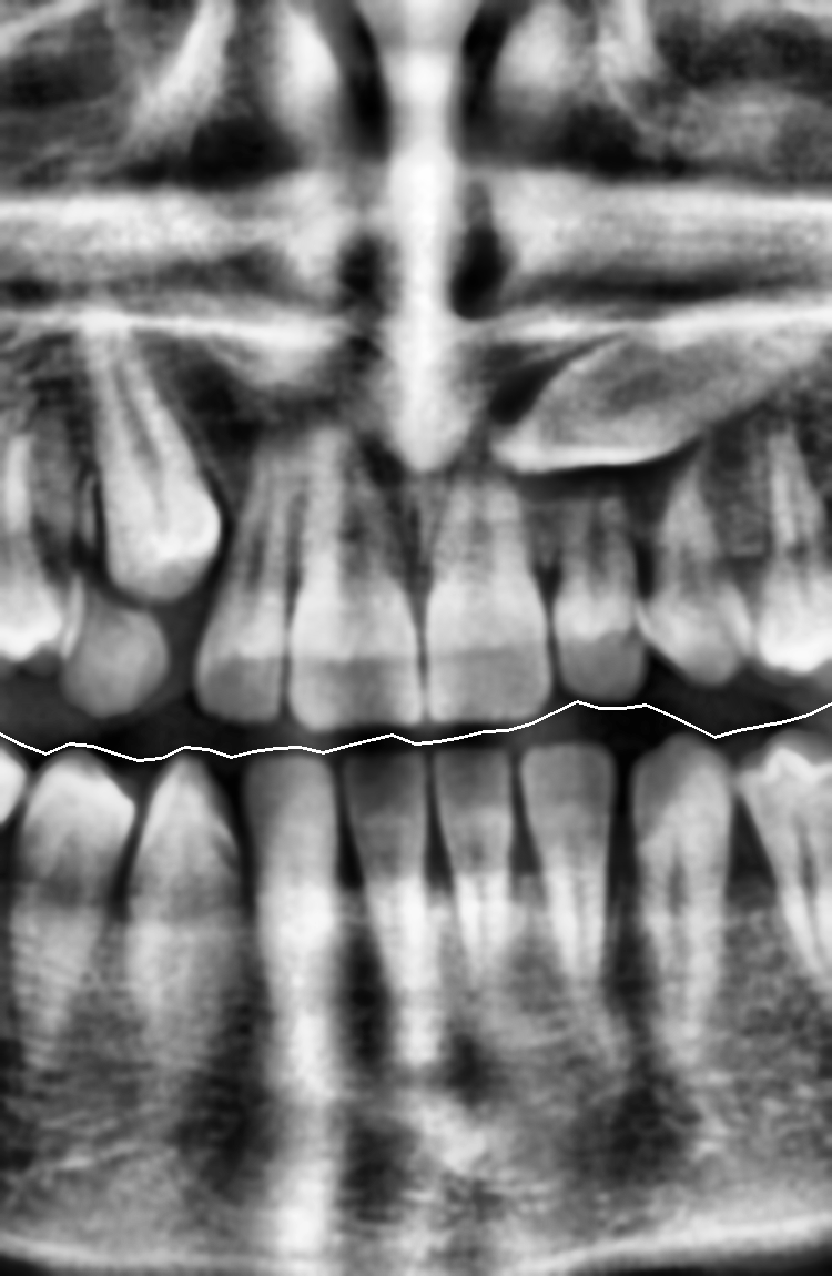
\includegraphics[width=5cm]{jawSplitLine-easy.png}}}
    \qquad
    \subfloat[]{{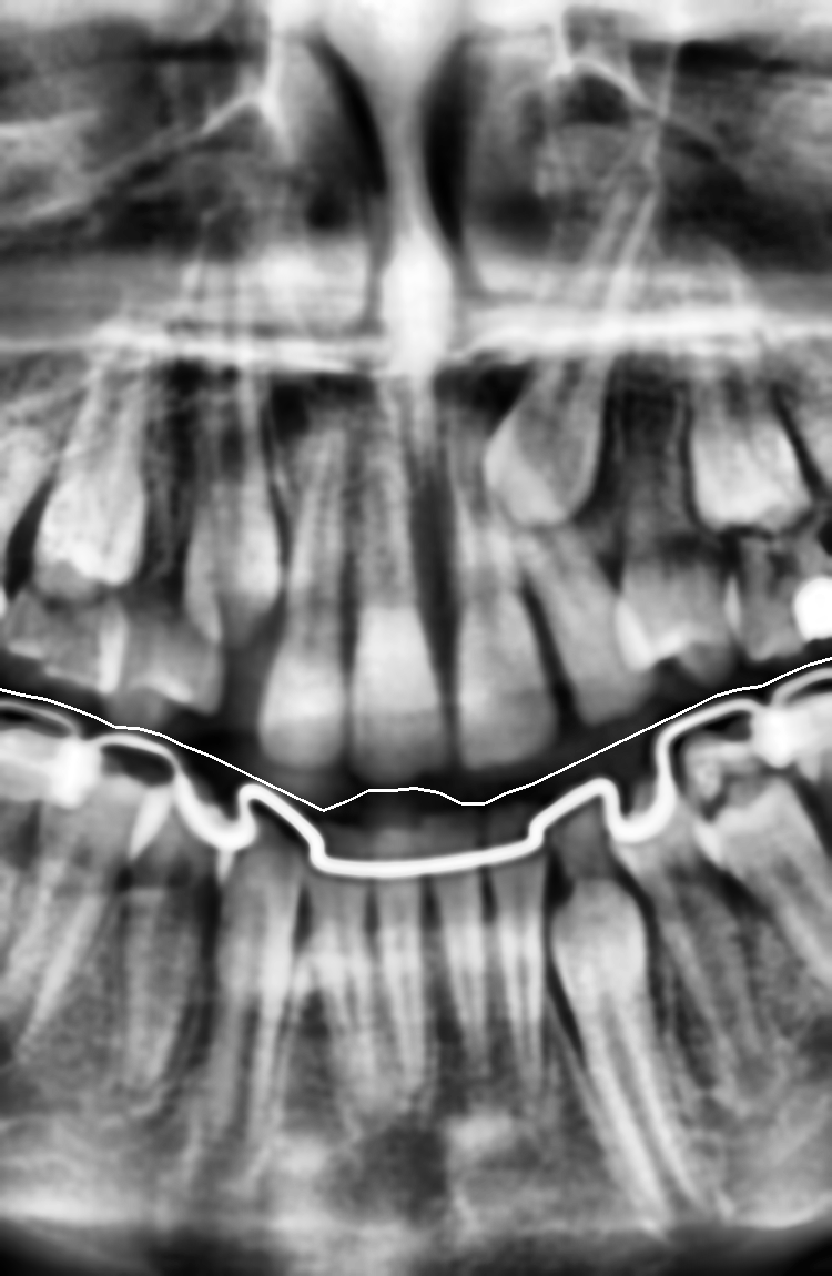
\includegraphics[width=5cm]{jawSplitLine-harder.png} }}
    \caption{Left, a simple jaw split line. Right, a more complicated one that follows the curve of the mouth.}
  \label{fig:jawSplitLine}
\end{figure}
\bigskip

The $x$ center of each mouth is simply approximated by the middle $x$ position of the image.
This means that the $x$ centers will not be accurate for regions of interest in which the mouth is shifted significantly to the left or to the right.
However, we noticed that most of the radiographs are nicely centered horizontally, which makes the middle $x$ position a good approximation.
The vertical center of each mouth is approximated by using the mean $y$ value of the jaw split line.
Note that in contrast to the $x$ center, simply approximating the $y$ center by the middle y position would be much less accurate.
This can be seen in figure~\ref{fig:jawSplitLine}, the mean $y$ position would be well above the $y$ center of each mouth.
The use of the jaw split line allows us to more accurately estimate the $y$ center, even if this $y$ center is different across images.

\subsection{Model for the upper and lower incisors}
\label{subsect:upper-lower-incisors}
The first initialization approach makes use of two statistical models. 
One for the upper four incisors and one for the lower four incisors.
To initialize these two models, we first locate the center of the mouth by using the method described above.
Once the center has been determined, we determine the origin of these models as follows:
\begin{itemize}
\item For the upper incisor model, we initialize the center of this model at a distance $d_u$ above the mouth center.
This distance $d_u$ is defined as the half of the mean length of the upper incisor teeth in the training data.
\item For the lower incisor model, we initialize the center of this model at a distance $d_l$ below the mouth center.
This distance $d_l$ is defined as the half of the mean length of the lower incisor teeth in the training data.
\end{itemize}
Once these models have been placed we apply the ASM algorithm until convergence.
The location of these models when they have been converged will be the start location of the individual tooth models.

\subsection{Multi Resolution Active Shape Model}
\label{subsect:multi-res}
Aside from the initialization model described above, a multi resolution search approach was also implemented as described in~\cite{Cootes1992AnIT}. 
In this case an ASM is trained for all eight incisor teeth at once.
Landmarks thus consist of 320 landmark points ($40\ points \times 8\ teeth$).
This approach makes use of a Gaussian pyramid as described in subsection~\ref{subsect:gaussian-pyramid}. 
Such a pyramid is built for each train and test image. 

The multi resolution active shape model is built as follows.
First, grey level models (subsection~\ref{subsect:grey-level-models}) are trained for each landmark point at each resolution level in the pyramid. 
Procrustes analysis is then performed to normalize the landmarks, and to find the mean landmark, scale, and rotation.
To finish building the model, PCA is performed on the normalized landmarks (subsection~\ref{subsect:pca}) and the resulting eigenvalues and eigenvectors are stored. 
The mean landmark and the eigenvectors are used in the search procedure to reconstruct landmarks. 
The eigenvalues are used to impose limits on the shapes of the landmarks that are reconstructed.

\subsubsection{Search Procedure}
For the detection of incisor teeth, the search procedure is started at the highest resolution level (i.e. lowest resolution image) in the Gaussian pyramid.
A low resolution version of the mean landmark is placed at the center of the mouth (found by the approach described in subsection~\ref{subsect:center of mouth}) and is then iteratively improved (as described in section~\ref{sect:asm}) until convergence or the maximum amount of iterations is reached.
The grey level model trained for the current resolution level is used in each iteration to find better landmark points.
Convergence is reached when the shape distance between two successive landmarks is less than 3.
After convergence, the landmark is scaled up (all points multiplied by 2) and moved one resolution level lower.
This is repeated until convergence is reached at the lowest level in the pyramid.
The resulting landmark can then be used for segmentation of teeth.

An example of the multi resolution search approach can be seen in figure~\ref{fig:multi-resolution-search-example}.
The radiograph used for the figure has no landmarks and thus was not used in the training of the model used for incisor detection. 
Figure~\ref{fig:multi-resolution-search-example} (a) shows the start of the search procedure, with the white polygons representing the mean landmark placed on the detected center of the mouth. 
As described above, the procedure is started at the highest resolution level in the Gaussian pyramid. 
Figure~\ref{fig:multi-resolution-search-example} (b) shows the same landmark after it has converged on the highest resolution level. 
Figure~\ref{fig:multi-resolution-search-example} (c) shows the same landmark after convergence on the original radiograph image.

\begin{figure}[!tbp]
  \centering
  \begin{adjustbox}{center}
    \subfloat[]{{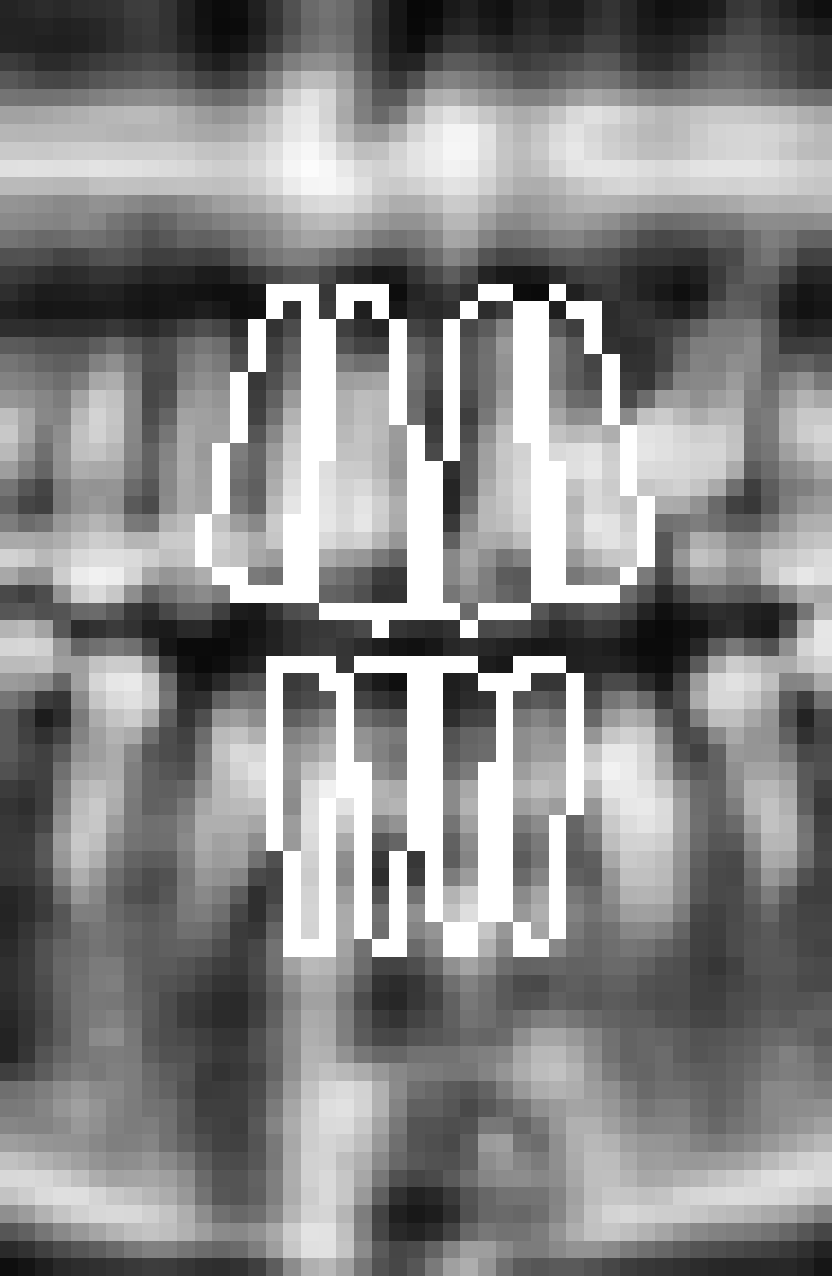
\includegraphics[width=5.5cm]{multi-resolution-24-init} }}
    \subfloat[]{{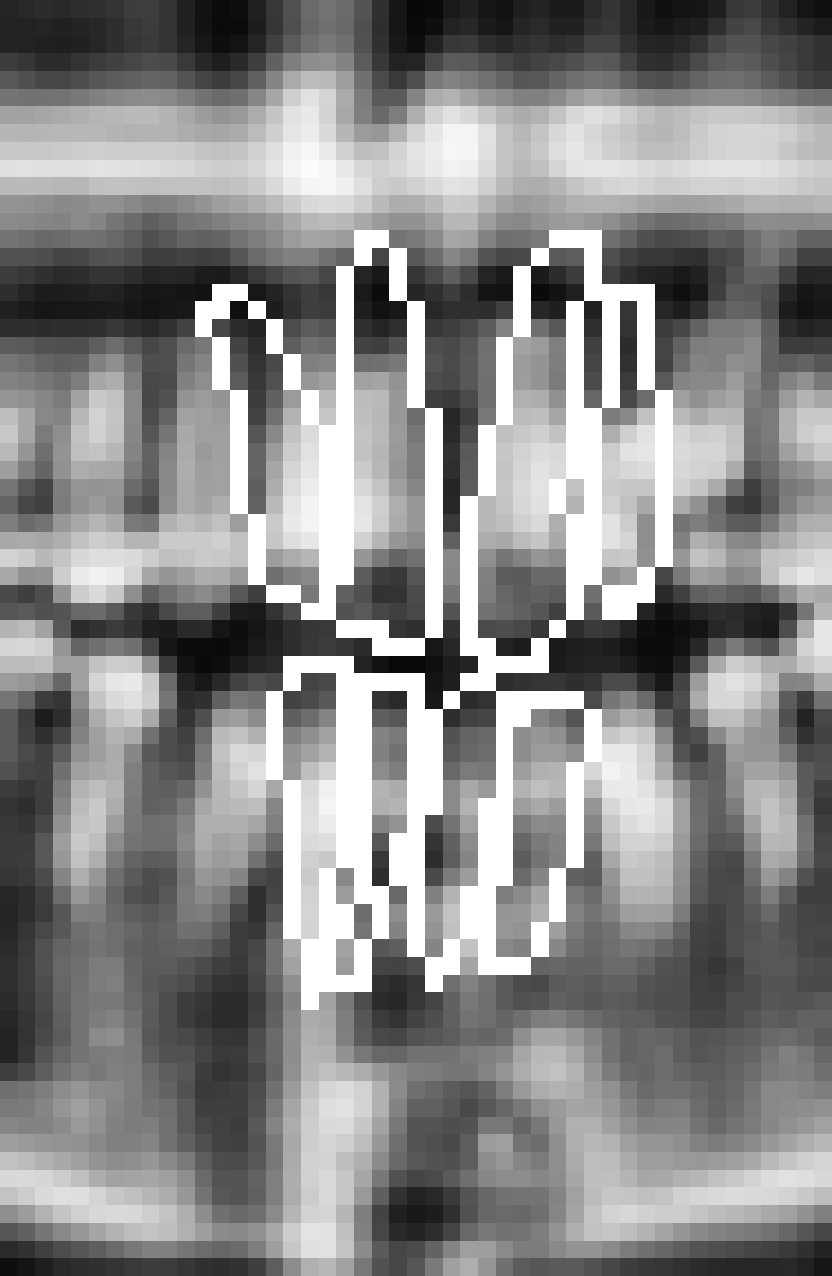
\includegraphics[width=5.5cm]{multi-resolution-24-init-converged} }}
    \subfloat[]{{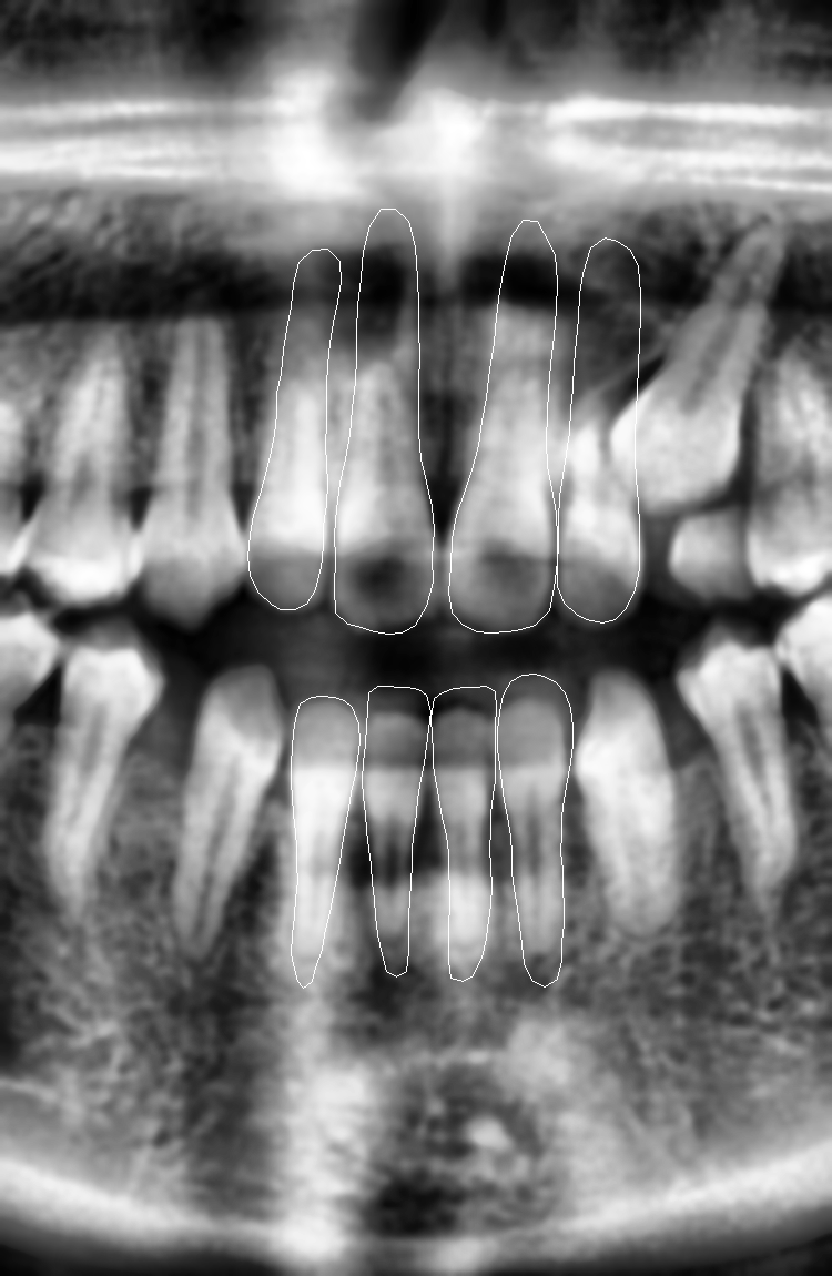
\includegraphics[width=5.5cm]{multi-resolution-24-final-converged} }}
  \end{adjustbox}
  \caption{The multi resolution ASM search approach applied to the radiograph with filename ``24.tif''.}
  \label{fig:multi-resolution-search-example}
\end{figure}

The multi resolution search approach simplifies the initialization procedure. 
At the highest level of the Gaussian pyramid, small movements correspond to large movements at the lowest level. 
The result of this is that small movements of a landmark on the lowest resolution image can place it on a good initial position for the higher resolution image on the pyramid level below it. In the higher resolution image, the location of the landmark is then refined more and passed further to higher resolution images.
Furthermore, this means that multi resolution search is able to shift landmarks both horizontally and vertically by a lot so that the models can still move to correct positions when the approximated center of the mouth lies far from the actual center.

\subsubsection{PCA}
In this approach, landmarks consist of many more points than when modeling teeth individually. 
This posed a problem for the eigenvectors that were obtained after PCA was performed on the landmarks. 
Reconstructions of these landmarks were much less accurate and were more crinkly than smooth. 
This effect can be seen in figure~\ref{fig:pca} (a).
An approach used to remedy this was to split each landmark up into eight landmarks and perform PCA for each tooth. 
Reconstructions were then made separately for each tooth and grouped back together into landmarks that contained all eight teeth. 
While this did cause the reconstructions to be much more smooth, it also caused teeth to overlap often, since they were reconstructed separately. 
A benefit of performing PCA on all teeth together is that the reconstructed landmarks then force the teeth to not overlap. 

Another approach to remedy this problem, the one that we ended up using, is to mirror all radiographs and their landmarks in order to double the training data. 
After performing PCA on the set of original and mirrored radiographs, reconstructions were much smoother, while still being able to adapt to new shapes found in improvement iterations, and still keeping teeth from overlapping. The result of this is visible in figure~\ref{fig:pca} (b).

\begin{figure}[!tbp]
  \centering
  \begin{adjustbox}{center}
    \subfloat[]{{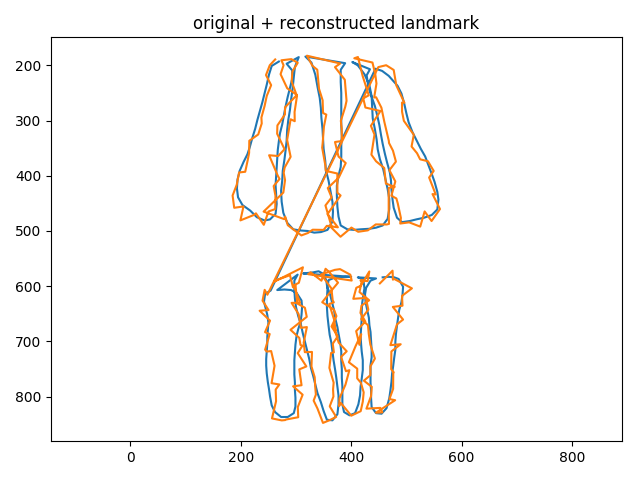
\includegraphics[width=8cm]{pca-crinkly} }}
    \subfloat[]{{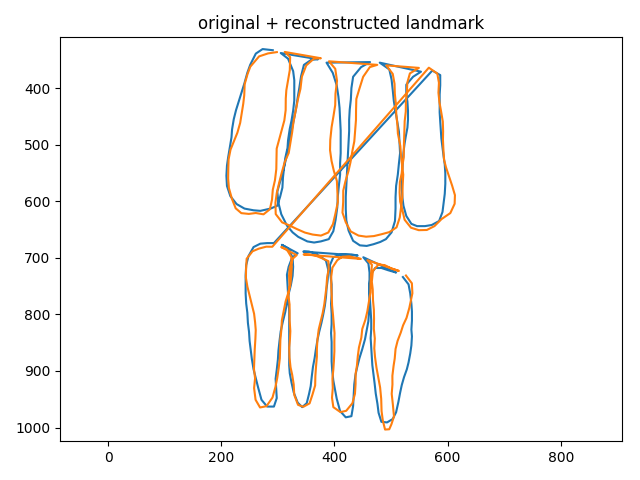
\includegraphics[width=8cm]{pca-pretty} }}
  \end{adjustbox}
  \caption{Reconstructions after PCA is performed on landmarks that consist of all eight teeth. Left, a reconstruction using the learned eigenvectors using all 14 radiographs, right, using all 14 radiographs and their mirrored versions.}
  \label{fig:pca}
\end{figure}

\newpage
\subsubsection{Parameters}
The following parameters were set for the multi resolution search experiments: 
\begin{itemize}
\item resolution levels = 5
\item maximum number of iterations allowed at each level = 20
\item number pixels on either side of point for grey level model = 7
\item number of sample points on either side of point for improvement search = 3
\item PCA components retained = 25. 
\end{itemize}
These parameters were chosen based on subjective evaluation of performance. A better way to choose parameters would be by using a parameter optimization method such as grid search or Bayesian optimization, but in the limited time for this project we did not do this.

\section{Evaluation}
\label{sect:evaluation}
To evaluate the performance of our approaches formally, the landmarks produced by search procedures are used to create segments of teeth.
These segments are then compared to \textit{ground truth} segments which we received with the assignment.
For the actual performance metrics, we have decided to use accuracy, precision, and recall.
These performance metrics are defined in terms of true positives (TP), false positives (FP), true negatives (TN), and false negatives (FN).
These terms are defined as follows in this project.
\begin{itemize}
\item \textbf{True Positive:} The model correctly predicts that a pixel is part of the incisors.
\item \textbf{False Positive:} The model incorrectly predicts that a pixel is part of the incisors.
\item \textbf{True Negative:} The model correctly predicts that a pixel is not part of the incisors.
\item \textbf{False Negative:} The model incorrectly predicts that a pixel is not part of the incisors.
\end{itemize}

The performance metrics are then defined as follows.
\begin{align} 
accuracy &= \frac{TP + TN}{TP + TN + FP + FN} \\ 
precision &= \frac{TP}{TP + FP} \\ 
recall &= \frac{TP}{TP + FN}
\end{align}
A drawback of using accuracy in this context is that it will always be high.
This is caused by the fact that most of the pixels in the binary segmentation images are black, which causes TN to be significantly higher than the other counts.
Since accuracy has TN both in the numerator and denominator, it will always be high.
Precision and recall avoid this effect by not using TN in their definitions.

\subsection{Leave One Out Cross-Validation}
\ldots



\section{Experiments}
\label{sect:experiments}
For the experiments, we report the average accuracy, precision, and recall of the leave one out cross-validation experiments.
In the appendix we provide an overlay for some of the test images.

\section{Neural Networks}
\label{sect:nns}
Although Neural networks were not part of the assignment we still decided to test them out even with the very limited data we had.
The last couple of years convolutional neural networks (CNN) have successfully been used in image recognition tasks.
For this reason we have decided to test two different CNN architectures.
The first CNN we tried is the YOLO\cite{yolov3} network that can draw bounding boxes around the objects of interest.
The second CNN we tried is the Mask-RCNN\cite{MASK-RCNN} network which creates masks to annotate the found objects.
Both networks have been trained on the fourteen training images that came with this project and have been initialized with pretrained weights (YOLO has pretrained darknet weights and Mask-RCNN has pretrained imagenet weights).
To train each of these networks we manually labeled the two incisor groups present on each of these fourteen images.
When we tested the YOLO network we didn't get a singly bounding box back, not even on the training dataset.
With the Mask-RCNN network however we got the following results:



\section{Conclusion}
\label{sect:conclusion}
\ldots



\newpage
\section{Appendix}
\label{sect:appendix}
\ldots



\bibliographystyle{plain}
\bibliography{sample}

\end{document}